\problemname{Magic Star}
A magic star consists of all the numbers from $1$ to $12$ arranged in the shape of a hexagram:

\begin{figure}[h]
	\centering
	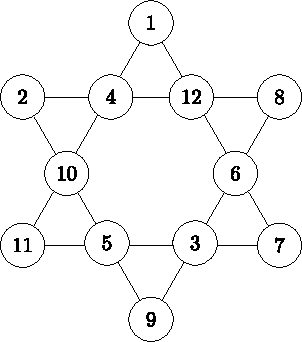
\includegraphics[width=0.35\textwidth]{sample}
\end{figure}

The magic comes from the fact that in each line of $4$ numbers, the sum of the numbers is $26$.
In the example given above, the six lines consist of the following numbers:
\begin{itemize}
	\item $1+4+10+11$
	\item $11+5+3+7$
	\item $7+6+12+1$
	\item $2+10+5+9$
	\item $9+3+6+8$
	\item $8+12+4+2$
\end{itemize}
There are several possible ways to arrange the numbers to get a magic star.
Given a partially labelled star, your task is to extend the solution such that a magic star is formed.

\begin{Input}
    The input consists of a visualization of the star;
    the unlabelled fields of the star will be represented by an `x' character, and labelled fields will contain a letter between `A' and `L', where the $i$-th letter in the alphabet represents number $i$.
    The character `.' is used to align the fields of the star in the shape of a hexagram.
    You may assume that each input will use the same alignment of the fields as the one in the sample input.
\end{Input}

\begin{Output}
    Print the lexicographically smallest extension of the given partial solution which is a magic star (lexicographically smallest means that the concatenation of the rows should result in a string which is lexicographically smaller than other potential solutions).
    You may assume that there is always a solution for the given input.
\end{Output}
